\section{Decision Tree}
In decision analysis, a decision tree can be used to visually and explicitly represent decisions and decision making. In data mining, a decision tree describes data (but the resulting classification tree can be an input for decision making).
\begin{itemize}
    \item Classification trees: Tree models where the target variable take a discrete set of values; in these tree structures, leaves represent class labels and branches represent conjunctions of features that lead to those class labels. 
    \item Regression trees: Decision trees where the target variable can take continuous values (typically real numbers). 
\end{itemize}
The term Classification And Regression Tree (CART) analysis is an umbrella term used to refer to both them.

Some techniques, often called ensemble methods, construct more than one decision tree:
\begin{itemize}
    \item Boosted tree: Incrementally building an ensemble by training each new instance to emphasize the training instances previously mis-modeled. A typical example is AdaBoost.
    \item Bootstrap aggregated (or bagged): decision trees, an early ensemble method, builds multiple decision trees by repeatedly resampling training data with replacement, and voting the trees for a consensus prediction, e.g., random forest.
    \item Rotation forest: in which every decision tree is trained by first applying principal component analysis (PCA) on a random subset of the input features
\end{itemize}

The basic algorithm used in decision trees is known as the ID3 (by Quinlan) algorithm. The ID3 algorithm builds decision trees using a top-down, greedy approach. Briefly, the steps to the algorithm are: Select the best attribute $\rightarrow$ Assign A as the decision attribute (test case) for the NODE. - For each value of A, create a new descendant of the NODE. - Sort the training examples to the appropriate descendant node leaf. - If examples are perfectly.

Now, the next big question is how to choose the best attribute. For ID3, we think of the best attribute in terms of which attribute has the most information gain, a measure that expresses how well an attribute splits that data into groups based on classification.

Pseudocode: ID3 is a greedy algorithm that grows the tree top-down, at each node selecting the attribute that best classifies the local training examples. This process continues until the tree perfectly classifies the training examples or until all attributes have been used.

The pseudocode assumes that the attributes are discrete and that the classification is binary. Examples are the training example. Target attribute is the attribute whose value is to be predicted by the tree. Attributes is a list of other attributes that may be tested by the learned decision tree. Finally, it returns a decision tree that correctly classifies the given Examples.

\subsection{Information Gain}
Information gain is a statistical property that measures how well a given attribute separates the training examples according to their target classification. As you can see in the Fig. , attribute with low information gain (right) splits the data relatively evenly and as a result doesn't bring us any closer to a decision. Whereas, an attribute with high information gain (left) splits the data into groups with an uneven number of positives and negatives and as a result helps in separating the two from each other.

% Fig \Cref{fig:info_gain}

% \begin{figure}[h]
%     \centering
%     \begin{subfigure}{.4\textwidth}
%         \centering
%         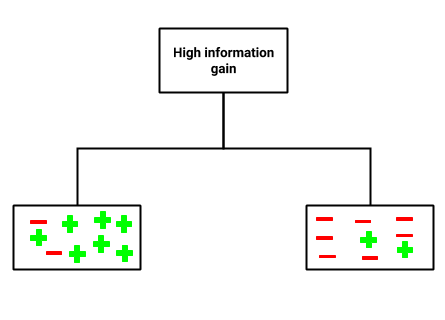
\includegraphics[scale=.45]{./images/decision_tree/high_gain.png}
%         \caption{High information gain.}
%         \label{fig:high_gain}
%     \end{subfigure}
%     \begin{subfigure}{.4\textwidth}
%         \centering
%         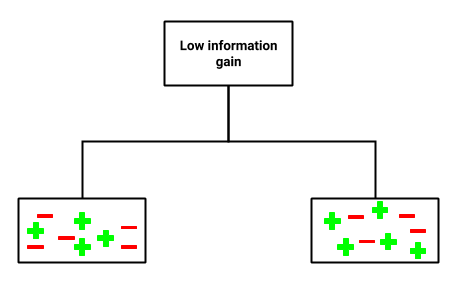
\includegraphics[scale=.45]{./images/decision_tree/low_gain.png}
%         \caption{Low information gain.}
%         \label{fig:low_gain}
%     \end{subfigure}
%     \caption{Information gain comparison.}
%     \label{fig:info_gain}
% \end{figure}

To define information gain precisely, we need to define a measure commonly used in information theory called entropy that measures the level of impurity in a group of examples. Mathematically, it is defined as:
$$Entropy = -\sum_i p_i \log p_i$$
, where $i$ is the class index. Since, the basic version of the ID3 algorithm deal with the case where classification are either positive or negative, we can define entropy as:
$$Entropy(S) = -p_+\log_2 p_+ - p_-\log_2 p_-$$
, where 
\begin{itemize}
    \item $S$: training examples
    \item $p_+$: is the proportion of positive examples in $S$
    \item $p_-$: is the proportion of negative examples in $S$
\end{itemize}

To illustrate, suppose $S$ is a sample containing 14 boolean examples, with 9 positive and 5 negative examples. Then, the entropy of $S$ relative to this boolean classification is:
$$Entropy([9+, 5-]) = -(9/14)\cdot \log_2(9/14) - (5/14)\cdot \log_2(5/14) = 0.940$$
Note that entropy is 0 if all the members of $S$ belong to the same class. For example, if all members are positive ($p_+$=1), then $p_-=0$, and $Entropy(S) = -1\cdot \log_2(1) -0\cdot \log_2(0) = 0$. Entropy is 1 when the sample contains an equal number of positive and negative examples. If the sample contains unequal number of positive and negative examples, entropy is between 0 and 1. The following figure shows the form of the entropy function relative to a boolean classification as $p_+$ varies between 0 and 1.

\begin{figure}[h]
    \centering
    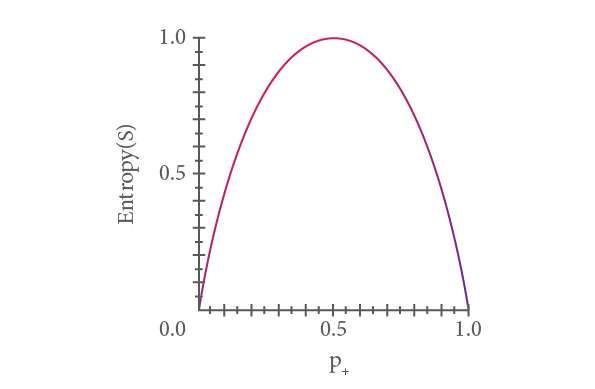
\includegraphics[scale=.40]{./images/decision_tree/entropy.jpg}
    \caption{Entropy.}
    \label{fig:entropy}
\end{figure}

Now, given entropy as a measure of the impurity in a sample of training examples, we can now define information gain as a measure of the effectiveness of an attribute in classifying the training data. Information gain, $Gain (S, A)$ of an attribute $A$, relative to a sample of examples $S$, is defined as:
$$Gain(S, A) \equiv Entrpoy(S) - \sum_{v \in Values(A)} \frac{|S_v|}{|S|} \cdot Entropy(S_v)$$
, where $|S_v|$ is a sample belongs to class $v$ and $|S|$ is the number of training samples. In other words,
$$\textrm{Gain  = Parent node of Entropy - [Average of Children Nodes Entropy]}$$
